\subsection{Experimentación ImagenFantasma con enteros}
\subsubsection{Hipótesis}
Este experimento consiste en realizar todos los cálculos posibles usando instrucciones que del tipo entero para cada pixel.
¿Por qué hacer esto? Bueno, las operaciones en enteros son usualmente más sencillas para el microprocesador, aunque trabajar de varios datos a la vez de seguro tiene un costo que de a un sólo dato, pero en cuanto al números de operaciones que se deberán realizar tiene mayor rendimiento.
A la hora de hacer cuentas, debido a los límites de una computadora en términos de precisión y tamaño de los datos que almacena, la hipótesis que es menos costoso y más rápido procesar números enteros que datos de punto flotante.
Además la idea surge porque los componentes de los pixeles son valores enteros (de 8 bits cada uno) y entonces de seguro no es necesario hacer todas sus operaciones en float, como el cálculo de b:
\begin{codesnippet}
\begin{verbatim}
        float b = (src_matrix[ii][jj].r + 2 * src_matrix[ii][jj].g + src_matrix[ii][jj].b) / 4;
\end{verbatim}
\end{codesnippet}
Esas operaciones se pueden hacer con operaciones de enteros, quizás se pierda algún dato al momento de la división. Quizás valga la pena en cuanto al rendimiento.
Entonces ¿Hay diferencias entre operar con enteros o punto flotantes? ¿Hay diferencias significativas en la imagen final? ¿Qué implementación es mejor?


\subsubsection{Resultados}
Con los datos obtenido de los tiempo de ejecución se realizaron los siguientes gráficos:

\begin{figure}[hb]
    \begin{center}
	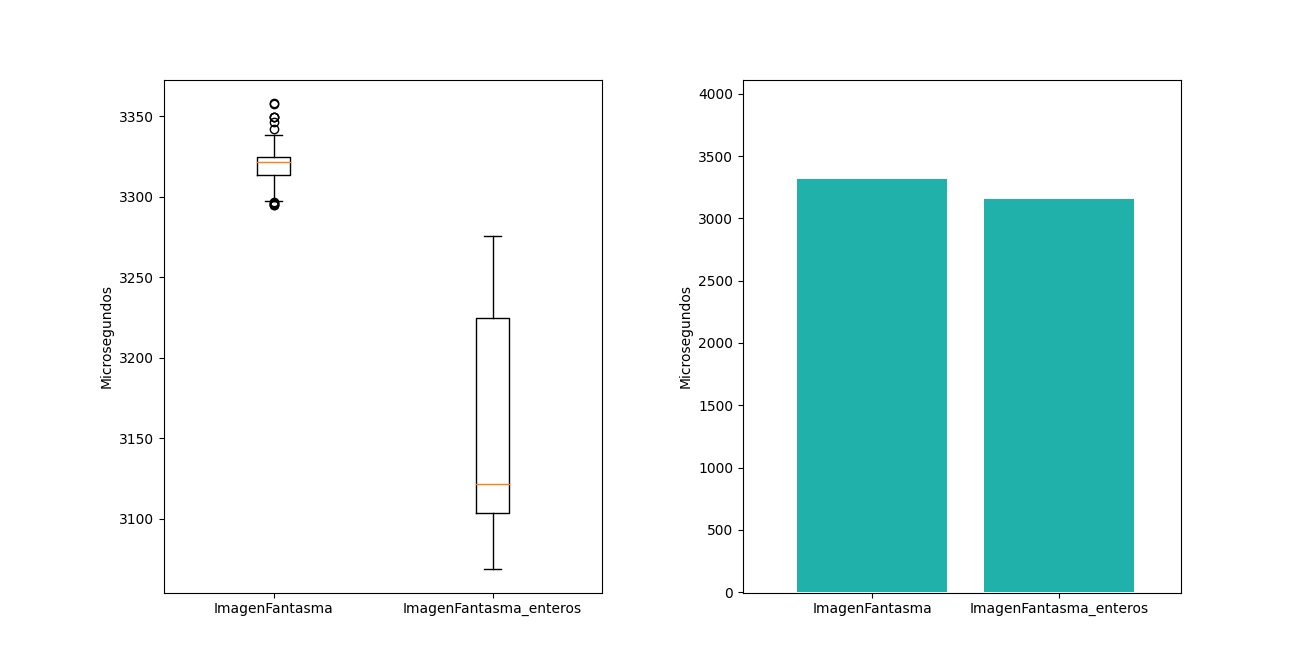
\includegraphics[scale=0.50]{img/enteros1.jpeg}
	\end{center}
	\caption{Dispersión y media microsegundos por ejecución}
	\label{exp1_m}
\end{figure}

Viendo el gráfico izquierdo, podríamos decir que no se ve una gran diferencia, ya que no tenemos una percepción justa en tiempo tan pequeños, pero viendo el gráfico de la derecha se puede decir que son bastante similares, la diferencia más o menos de 200 microsegundos es despreciable.

\begin{figure}
    \begin{center}
	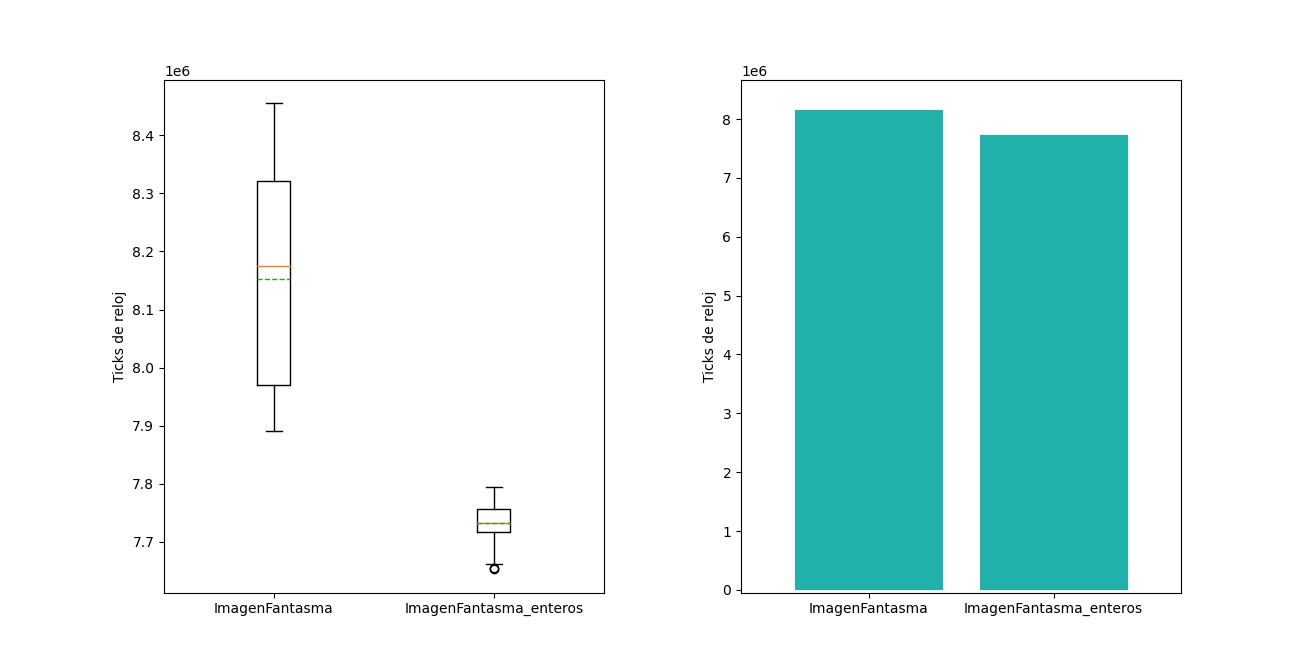
\includegraphics[scale=0.50]{img/enteros2.jpeg}
    \end{center}
	\caption{Dispersión y media de los ticks de reloj}
	\label{exp1_c}
\end{figure}

Pero con el gráfico de los ticks reloj se puede apreciar un poco más las diferencias dado que son más cuantificables. Los boxplot muestran que las operaciones con float llevan a que los tiempos tengan una media de poco más 8 millones en mayor parte. En cuanto a las operaciones en enteros los valores rondan por debajo de los 8 millones, con una media de alrededor de los 7.75 millones de ticks de reloj.

\subsubsection{Conclusión}
Dado los resultados se concluye que la hipótesis es correcta, como se esperaba. Aunque no se ve una diferencia muy grande, ambas implementaciones tienen un comportamiento similar.
Probablemente se deba al siguiente extracto del pseudocódigo:
\begin{codesnippet}
\begin{verbatim}
    dst_matrix[i][j].r = SATURAR(src_matrix[i][j].r * 0.9 + b/2);
    dst_matrix[i][j].g = SATURAR(src_matrix[i][j].g * 0.9 + b/2);
    dst_matrix[i][j].b = SATURAR(src_matrix[i][j].b * 0.9 + b/2);
\end{verbatim}
\end{codesnippet}
El multiplicar por 0.9, que es un número flotante, es una operatoria que no podemos realizar con números enteros y tampoco existe una instrucción que divida con enteros en \textbf{SIMD}, es por eso que a pesar del cálculo de b se haya realizado con operaciones en enteros aún se tuvo que extender cada componente de los pixeles a tamaños de 4 bytes para luego convertirlos en floats y luego volver a convertirlos en enteros, y reducirlos a tamaño byte, en toda ese proceso es donde creo que se encuentra el límite de la mejora de performance para esta implementación.
